\clearpage


\begin{SCfigure}
  \centering
  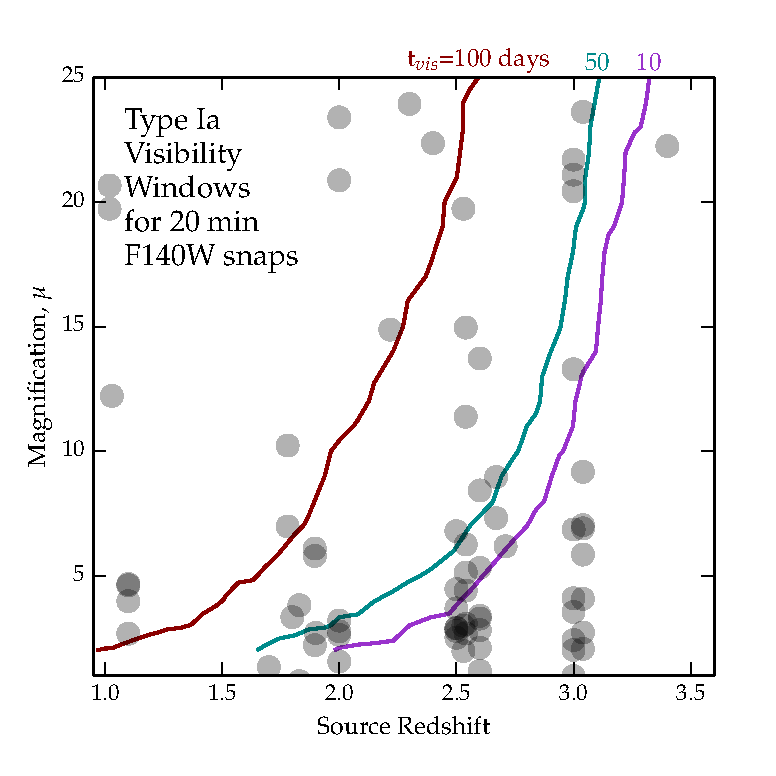
\includegraphics[width=0.5\textwidth]{FIG/tvis_muz_20min.pdf}
  \caption{ \label{fig:tvis}
Visibility time contours in the redshift-magnification plane.  For any
given redshift and magnification, we estimate $t_{vis}$, the number of
days that an average \SNIa\ would be detectable in a 20-minute
snapshot.  Solid lines plot contours of constant visibility time in
the $z-\mu$ plane at $t_{vis}=$100, 50, and 10 days.  Grey circles
mark the magnifications and redshifts for 50 strongly-lensed galaxy
images from three of our primary cluster targets.  Thus, if a galaxy
lies to the left of the 50-day line, then it is visible to our survey
for at least 50 days. }
\end{SCfigure}


\begin{figure}
  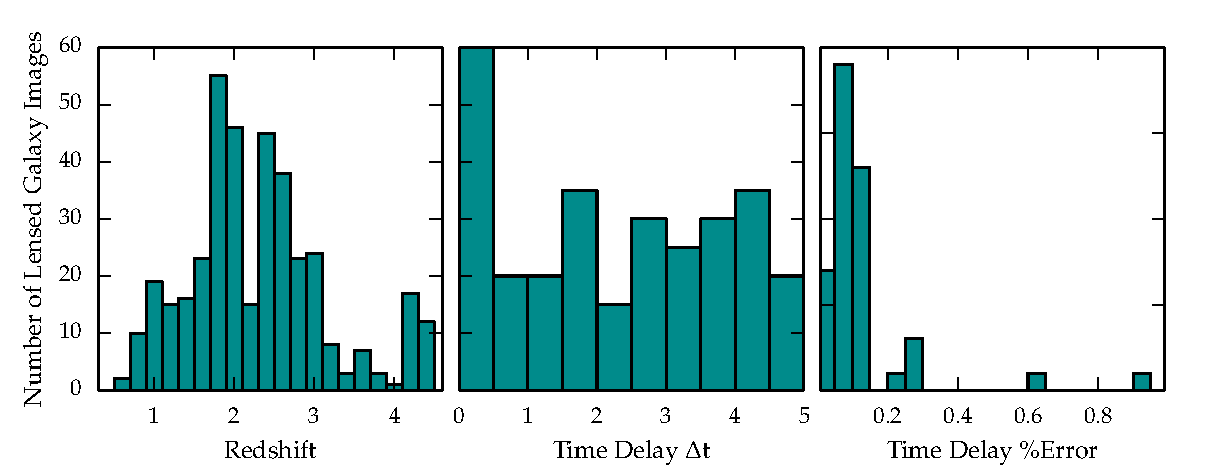
\includegraphics[width=\textwidth]{FIG/histograms.pdf}
  \caption{ \label{fig:tvis} Histograms showing the distribution of a
    representative sample of lensed galaxy images over redshift
    (left), time delay (middle) and time delay precision (right). 
}
\end{figure}

